%---------------------------------------------------------------------
%
%                          Cap�tulo 4
%
%---------------------------------------------------------------------
%
% 04Imagenes.tex
% Copyright 2009 Marco Antonio Gomez-Martin, Pedro Pablo Gomez-Martin
%
% This file belongs to the TeXiS manual, a LaTeX template for writting
% Thesis and other documents. The complete last TeXiS package can
% be obtained from http://gaia.fdi.ucm.es/projects/texis/
%
% Although the TeXiS template itself is distributed under the 
% conditions of the LaTeX Project Public License
% (http://www.latex-project.org/lppl.txt), the manual content
% uses the CC-BY-SA license that stays that you are free:
%
%    - to share & to copy, distribute and transmit the work
%    - to remix and to adapt the work
%
% under the following conditions:
%
%    - Attribution: you must attribute the work in the manner
%      specified by the author or licensor (but not in any way that
%      suggests that they endorse you or your use of the work).
%    - Share Alike: if you alter, transform, or build upon this
%      work, you may distribute the resulting work only under the
%      same, similar or a compatible license.
%
% The complete license is available in
% http://creativecommons.org/licenses/by-sa/3.0/legalcode
%
%---------------------------------------------------------------------

\chapter{Implementaci\'on de las aplicaciones}
\label{cap4}
\label{cap:impl}

En este cap\'itulo se detalla todo el proceso de creaci\'on y desarrollo de las diferentes aplicaciones y la demo que posteriormente se utiliza como ejemplo de implementaci\'on de la herramienta.
Se ha divido este cap\'itulo en 3 secciones:

\begin {itemize}
\item Implementaci\'on de la aplicaci\'on de Android.
\item Implementaci\'on de la aplicaci\'on de Unity.
\item Inclusi\'on de la herramienta en un juego cerrado.
\end {itemize}

%-------------------------------------------------------------------
\section{Implementaci\'on de la aplicaci\'on de Android}
%-------------------------------------------------------------------

Este proyecto se ha desarrollado utilizando principalmente 2 tecnolog\'ias: el motor de Unity y Android. Al tratarse de un proyecto de creaci\'on de un controlador para videojuegos y tomando como base la especificaci\'on desarrollada en el cap\'itulo 3 se ha optado por el desarrollo de una aplicaci\'on para Android que sirva como dispositivo de entrada y una aplicaci\'on en Unity que sirva como ejecutor del juego.

Android Studio es el entorno de desarrollo integrado (IDE) oficial para la plataforma de Android. Hasta finales del 2014 para desarrollar en Android se utilizaba Eclipse como IDE oficial y est\'a disponible para las plataformas Microsoft Windows, macOS y GNU/Linux. Android Studio incluye una gran variedad de herramientas para facilitar el desarrollo en Android entre las que se incluyen:

\begin {itemize}
\item Plantillas para crear dise\~nos comunes de Android y otros componentes.
\item Un editor de dise\~no enriquecido que permite a los usuarios arrastrar y soltar componentes de la interfaz de usuario.
\item Soporte para construcci\'on basada en Gradle.
\item Un dispositivo virtual de Android que se utiliza para ejecutar y probar aplicaciones.
\item Consola de desarrollador: consejos de optimizaci\'on, ayuda para la traducci\'on y estad\'isticas de uso.
\item Integraci\'on de ProGuard y funciones de firma de aplicaciones.
\end {itemize}
 
Los lenguajes de programaci\'on aceptados por Android Studio son Kotlin, Java y C++. En concreto para este proyecto se ha usado Java como lenguaje de programaci\'on.

%-------------------------------------------------------------------
\subsection {Ciclo de vida de Android}
%-------------------------------------------------------------------

Las aplicaciones en Android se rigen por una serie de componentes que se llaman \textbf{\textit{Activity}}. Estos componentes son claves a la hora de manejar los estados de una aplicaci\'on en Android. A diferencia de otros paradigmas de programaci\'on que comienzan sus aplicaciones con un m\'etodo \textbf{\textit{main()}}, la instancia de una Actividad invoca m\'etodos de devoluci\'on de llamada que se corresponden con etapas espec\'ificas de su ciclo de vida. La experiencia de una aplicaci\'on para un dispositivo m\'ovil difiere mucho de la versi\'on de escritorio de esa misma aplicaci\'on ya que la interacci\'on del usuario con la aplicaci\'on no siempre comienza en el mismo lugar. Un claro ejemplo de esto sucede con las aplicaciones de mensajer\'ia instantanea. Un usuario puede estar navegando por cualquier red social y encontrarse una publicaci\'on interesante y compartirla por correo electr\'onico o por una aplicaci\'on de mensajer\'ia instantanea. La aplicaci\'on de correo electr\'onico no se abre en el mismo estado si se abre desde la opci\'on de compartir de la red social o si se abre desde el men\'u de aplicaciones instaladas en el dispositivo. Las Actividades est\'an dise\~nadas para facilitar este paradigma.

La mayor\'ia de las aplicaciones contienen varias pantallas, lo cual significa que contienen varias actividades. Este concepto se pondr\'a posteriormente de manifiesto ya que para el desarrollo de la aplicaci\'on han sido necesarias 2 Actividades. Una actividad proporciona una ventana en la que la aplicaci\'on dibuja la interfaz de usuario. Esta ventana puede estar a pantalla completa o puede ser m\'as peque\~na y flotar sobre otras ventanas como si fuese un \textit{pop-up}.

Cuando un usuario navega por una aplicaci\'on, la cierra, la vuelve a abrir o la minimiza, las instancias de las Actividades de la aplicaci\'on pasan por una serie de estados de su ciclo de vida. Estos estados pueden tener comportamientos definidos por los desarrolladores de la aplicaci\'on. Esto permite tener un control sobre lo que ocurre en cada uno de los estados de la aplicaci\'on. Para navegar por las transiciones entre las etapas del ciclo de vida de una actividad, la clase Activity proporciona un conjunto b\'asico de seis devoluciones de llamadas: \textbf{onCreate() ,onStart(), onResume(), onPause(), onStop() y onDestroy().} El sistema invoca cada una de estas devoluciones de llamada cuando una operaci\'on entra en un nuevo estado.


\begin{figure}[h]

\centering
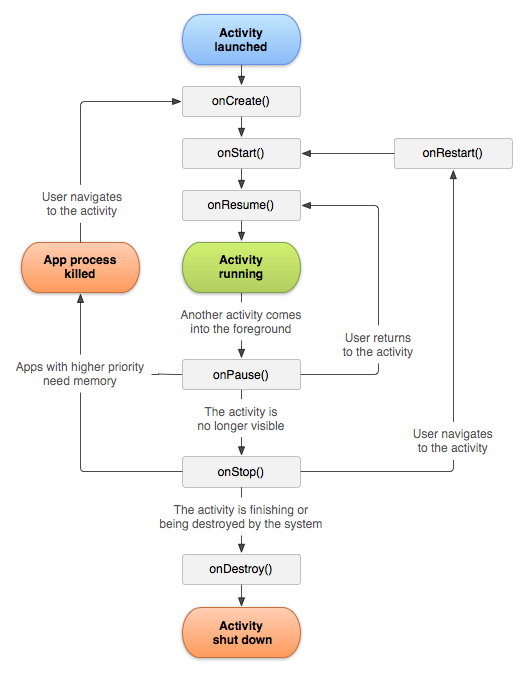
\includegraphics[width=0.7\textwidth]{./Imagenes/Bitmap/Ciclo_de_vida_Android}
\caption{Ciclo de vida de una Actividad de un sistema Android}
\end{figure}


Cada uno de los estados que tiene la actividad es llamado en un momento concreto de la ejecuci\'on de la Actividad. Las caracter\'isticas de cada uno de estos estados son las siguientes:

\begin {itemize}
\item \textbf{onCreate()} $\rightarrow$ Este m\'etodo es el primero que llama cuando se crea la Actividad. Este estado es utilizado para ejecutar la l\'ogica de la aplicaci\'on que debe ocurrir \'unicamente una vez en todo el ciclo de vida. Este m\'etodo recibe el par\'ametro \textit{\textbf{savedInstanceState}}, que es un objeto de tipo \textbf{\textit{Bundle}} que contiene el estado ya guardado de la actividad. Si la actividad nunca existi\'o, el valor del objeto \textit{Bundle} es nulo.
\item \textbf{onStart()} $\rightarrow$ Cuando la actividad entra en el estado Started, el sistema invoca esta devoluci\'on de llamada. La llamada \textit{onStart()} hace que el usuario pueda ver la actividad mientras la app se prepara para que esta entre en primer plano y se convierta en interactiva. Por ejemplo, este m\'etodo es donde la app inicializa el c\'odigo que mantiene la IU.
\item \textbf{onResume()} $\rightarrow$  La aplicaci\'on permanece en este estado hasta que ocurre alg\'un evento que la quita de foco. Tal evento podr\'ia ser, por ejemplo, recibir una llamada telef\'onica, que el usuario navegue a otra actividad o que se apague la pantalla del dispositivo.
\item \textbf{onPause()} $\rightarrow$ Este estado se utiliza cuando se ha perdido el foco de una aplicaci\'on. Sin embargo una actividad con el estado Paused puede ser completamente visible si est\'a en el modo multiventana. En este estado no deben guardarse datos de la aplicaci\'on ya que es un estado que dura poco tiempo.
\item \textbf{onStop()} $\rightarrow$ En este estado es donde los componentes del ciclo de vida pueden detener cualquier funcionalidad que no necesite ejecutarse mientras el componente no sea visible en la pantalla. Este estado debe usarse para liberar o ajustar recursos que no son necesarios mientras no sea visible para el usuario.
\item \textbf{onDestroy()} $\rightarrow$ Se llama a este m\'etodo antes de que se finalice la actividad. El sistema invoca esta devoluci\'on de llamada cuando el dispositivo rota o cuando la aplicaci\'on se cierra. En este estado es donde los componentes del ciclo de vida pueden recuperar cualquier elemento que se necesite antes de que finalice la Actividad.
\end {itemize}

%-------------------------------------------------------------------
\subsection {Arquitectura de la aplicaci\'on Android}
%-------------------------------------------------------------------

Para que la aplicaci\'on Android cumpla los requisitos expuestos en el apartado de especificaci\'on del proyecto, se han implementado 3 clases:

\begin {itemize}
\item \textbf{Controller} $\rightarrow$ Esta es la actividad principal. Desde esta actividad se recogen los datos de IP y puerto al que debe conectarse el dispositivo Android para ser utilizado como controlador.Al crearse la Actividad se lanza la ejecuci\'on de una hebra que se encargar\'a de recibir, leer e interpretar las im\'agenes que lleguen por red una vez la aplicaci\'on se conecte al juego. Desde esta clase se controla la pulsaci\'on del usuario en la pantalla. De esta pulsaci\'on se guardan 3 datos: posici\'on (x,y) donde se ha realizado la pulsaci\'on y el tipo de pulsaci\'on (presionar,levantar o arrastrar). Para cada una de estas pulsaciones se dispara la ejecuci\'on de hilo (\textbf{UdpClientThread}). La \'ultima funci\'on de esta clase es la de cambiar la imagen que se muestra en la aplicaci\'on. 
\item \textbf{UdpClientThread} $\rightarrow$ Esta clase tiene como funci\'on el env\'io de datos a la aplicaci\'on donde se ejecuta el juego. La primera vez que el usuario realice una pulsaci\'on se enviar\'a el tama\~no de la pantalla del dispositivo Android. Adem\'as de este mensaje, esta hebra se encarga del env\'io de paquetes que incluyen el tipo de pulsaci\'on que se ha realizado, la coordenada x y la coordenada y de la pantalla del dispositivo donde se ha realizado la pulsaci\'on. Una vez que la aplicaci\'on se cierre, el packete de cierre de conexi\'on se env\'ia desde esta hebra.
\item \textbf{Receive\_Image} $\rightarrow$ Esta clase se ejecuta desde una hebra distinta a la de la Actividad principal y la funci\'on que desempe\~na es la de recibir informaci\'on que mande el juego. Esta clase se queda escuchando en un puerto designado, normalmente el mismo que abre el juego para recibir los datos de la aplicaci\'on Android. Los primeros mensajes en llegar son el tiempo de vibraci\'on del dispositivo cada vez que se realice una pulsaci\'on en la pantalla y posteriormente las im\'agenes que se env\'ien desde el juego. Estas im\'agenes se esperan en formato PNG ya que se realiza una descompresi\'on de este formato.
\end {itemize}


\begin{figure}[h]

\centering
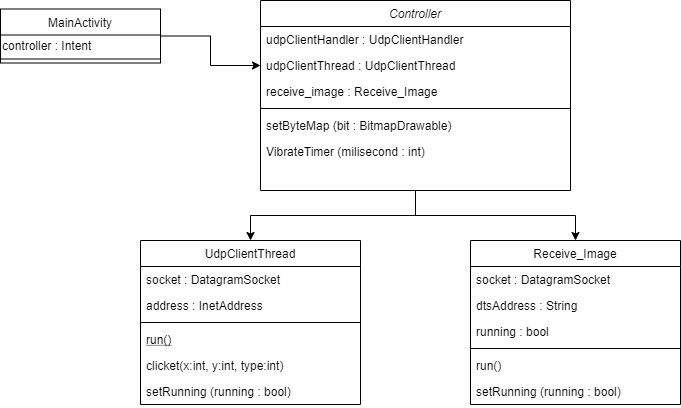
\includegraphics[width=0.8\textwidth]{./Imagenes/Bitmap/Arquitectura_App_Android}
\caption{Arquitectura de la aplicaci\'on Android implementada}
\end{figure}

Se ha optado por una aplicaci\'on cerrada para que el desarrollador no tenga que implementar nueva funcionalidad en Android. El coste computacional de la aplicaci\'on es bajo, lo que permite ser utilizado en una gran cantidad de dispositivos. La divisi\'on en 2 actividades es debido a que el flujo de Android se basa en ir cambiando entre actividades para que cada una tenga un uso espec\'ifico. La primera actividad de usa para capturar un QR con la c\'amara y la segunda es utilizada para simular un mando.

%-------------------------------------------------------------------
\section{Implementaci\'on de la aplicaci\'on de Unity}
%-------------------------------------------------------------------

Como se coment\'o al principio de este cap\'itulo, el motor de videojuegos elegido para la realizaci\'on de este proyecto ha sido Unity. Unity es un motor de videojuegos multiplataforma creado por \textit{Unity Technologies} en 2005. Unity est\'a disponible como plataforma de desarrollo para Microsoft, Mac OS y Linux y tiene soporte de compilaci\'on con m\'ultiples plataformas:

\begin {itemize}
\item \textbf{Web} $\rightarrow$ WebGL.
\item \textbf{PC} $\rightarrow$ Windows, SteamOS, Linux, OS X y Windows Store Apps.
\item \textbf{Dispositivos m\'oviles} $\rightarrow$ iOS, Android, Windows Phone.
\item \textbf{Smart TV} $\rightarrow$ tvOS, Samsung Smart TV, Android TV.
\item \textbf{Consolas} $\rightarrow$ PlayStation Vita, PlayStation 4, Xbox 360, Xbox One, Wii U, Nintendo 3DS, Nintendo Switch.
\item \textbf{Dispositivos de realidad virtual} $\rightarrow$ Oculus Rift, Google Cardboard, HTC Vive, PlayStation VR, Samsung Gear VR
\end {itemize}

Adem\'as de contar con soporte para m\'ultiples dispositivos, Unity puede usarse junto con m\'ultiples herramientas de desarrollo como \textbf{Blender}, \textbf{Autodesk 3ds Max} y \textbf{ZBrush} entre otros.

%-------------------------------------------------------------------
\subsection {Funcionamiento de Unity}
%-------------------------------------------------------------------

Unity es un motor de videojuegos que aglutina una gran variedad de herramientas para el desarrollo. Estas herramientas van desde inclusiones de \textbf{Scripts} para dar comportamientos espec\'ificos a cada una de las \textbf{Entidades} del juego hasta elementos m\'as visuales como diagramas de estado para el control de las animaciones de un modelo. Para que todos estos sistemas tan diferentes puedan convivir, hay una serie de funciones que se ejecutan en un orden determinado. Unity a su vez se compone de varios elementos clave:

\begin {itemize}
\item \textbf{Escena} $\rightarrow$  Las escenas contienen los objetos del juego. Pueden usarse para crear niveles, men\'us o cualquier estado del juego.
\item \textbf{GameObjects / Entidades} $\rightarrow$ Cada una de las escenas contiene objetos. Estos objetos se llaman GameObjects. Cualquier elemento es considerado un GameObject, no tiene por qu\'e tener una representaci\'on visual (m\'usica, c\'amara, etc).
\item \textbf{Componentes} $\rightarrow$ Los componentes son los diferentes atributos que se le dan a los GameObjects para que tengan funcionalidad (movimiento, posici\'on, animaci\'on, colisi\'on f\'isica, etc).
\end {itemize}

Unity ofrece una serie de componentes que dan una funcionalidad ya definida a un objeto, esta funcionalidad va desde tener una posici\'on definida en el mundo hasta emitir un sonido y realizar una animaci\'on. Los desarrolladores pueden desarrollar sus propios componentes usando Scipts. Estos scripts indican a las diferentes entidades c\'omo comportarse. El lenguaje seleccionado para este sistema de \textit{scripting} es C\# y un script debe estar vinculado a una entidad para que este se ejecute. Al tratarse de un sistema basado en la ejecuci\'on e interacci\'on entre scripts, Unity tiene una serie de funciones que se ejecutan autom\'aticamente por el motor. Estas funciones son:

\begin {itemize}
\item \textbf{Awake} $\rightarrow$  Awake se invoca solo una vez al inicio de la ejecuci\'on. Si un GameObject est\'a inactivo, entonces no podr\'a invocarse hasta que se le active. Sin embargo, Awake se invoca incluso si el GameObject est\'a activo pero el componente no est\'a habilitado. Se puede utilizar Awake para inicializar todas las variables a las que es necesario asignar un valor.
\item \textbf{Start} $\rightarrow$ Al igual que Awake, Start se invocar\'a si un GameObject est\'a activo, pero solo si el componente est\'a habilitado.
\item \textbf{Update} $\rightarrow$ Update se invoca una vez por frame. En esta funci\'on se debe definir la l\'ogica que se ejecuta continuamente, como animaciones, inteligencia artificial y otras partes del juego que tienen que actualizarse continuamente.
\item \textbf{FixedUpdate} $\rightarrow$ Esta funci\'on es muy similar a Update pero su uso queda reservado para el desempe\~no de acciones en las que est\'e involucrada la f\'isica. Unity tiene un sistema basado en frames y FixedUpdate es la \'unica funci\'on en la que se asegura que se va a ejecutar en un \textit{frame-rate} fijo. 
\item \textbf{LateUpdate} $\rightarrow$ Esta es una funci\'on que es similar a Update, pero LateUpdate se invoca al final del frame. Unity analizar\'a todos los objetos de juego, encontrar\'a todas las Updates, e invocar\'a las LateUpdates. Esto es bueno para entidades como la c\'amara.
\end {itemize}



%-------------------------------------------------------------------
\subsection {Arquitectura de la API en Unity}
%-------------------------------------------------------------------

Para que la aplicaci\'on desarrollada en Unity cumpla los requisitos expuestos en el apartado de especificaci\'on del proyecto, se han realizado 2 clases:

\begin {itemize}
\item \textbf{UDPSocket} $\rightarrow$ Esta clase se utiliza para la creaci\'on de todo lo necesario para hacer funcionar esta herramienta. Con el m\'etodo \textbf{init()} se inician 2 hebras de ejecuci\'on diferentes. Una de ellas se encarga de enviar los datos necesarios al dispositivo de entrada. Estos datos son tanto la vibraci\'on como la imagen a renderizar en el dispositivo. La otra se encarga de recibir los datos de entrada del dispositivo y avisar a los diferentes \textit{listeners}. Estos listeners utilizan esa informaci\'on para los prop\'ositos desigandos por el desarrollador del juego (mover al personaje, pausar el juego, salir, etc). Esta clase tambi\'en se encarga de cerrar la conexi\'on.
\item \textbf{InputMobileInterface} $\rightarrow$ Esta interfaz sirve para dar soporte a la conexi\'on.\textbf{ EndOfConnection()} debe ser utilizado para finalizar la conexi\'on. \textbf{ReceiveTouch()} recibe las coordenadas donde se ha realizado la pulsaci\'on en el dispositivo de entrada. La misi\'on de esta funci\'on es comprobar si estas coordenadas corresponden con la posici\'on de un bot\'on u objeto interactuable dentro del juego. Por \'ultimo \textbf{ScreenSize()} recibe las dimensiones del dispositivo de entrada para posteriormente poder enviar im\'agenes y hacer las transformaciones de la posici\'on de los botones.
\end {itemize}

\begin{figure}[h]

\centering
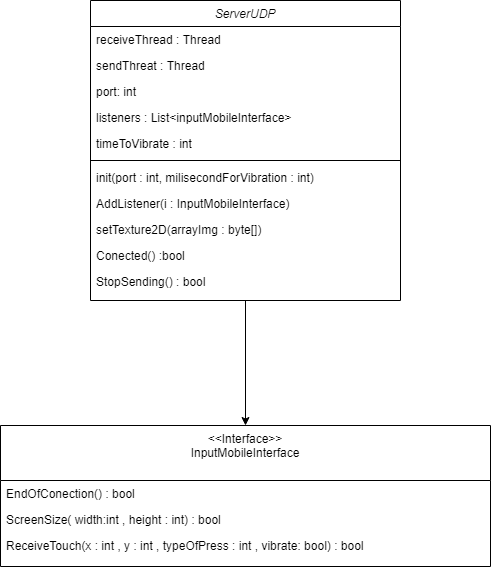
\includegraphics[width=0.8\textwidth]{./Imagenes/Bitmap/Arquitectura Unity}
\caption{Arquitectura de la aplicaci\'on de Unity implementada}
\end{figure}

Con esta implementaci\'on se quiere dar al desarrollador una API que permita al usuario tener un nivel de abstracci\'on superior al que tendr\'ia en caso de tener que manejar directamente la conexi\'on entre 2 dispositivos y el tratamiento de input. Esto se ha conseguido manejando los hilos de manera individual y a la funcionalidad dada por la interfaz \textbf{InputMobileInterface}. La interfaz permite que el desarrollador decida en cada momento de la ejecuci\'on lo que se realiza en cada una de sus fases.

La primera fase consiste en el reescalado de las im\'agenes que se env\'ian. En la segunda fase se realiza el tratamiento del input. En esta fase el desarrollador deber\'a decidir las coordenadas de los botones que quiere que tenga su mando y decidir qu\'e acci\'on se va a realizar con la pulsaci\'on de estos botones. La \'ultima fase involucra volver a lanzar el servidor en caso de que se pierda la conexi\'on ya sea porque el dispositivo se apaga, porque se cierre la conexi\'on de manera controlada o por inactividad.

% Variable local para emacs, para  que encuentre el fichero maestro de
% compilaci�n y funcionen mejor algunas teclas r�pidas de AucTeX
%%%
%%% Local Variables:
%%% mode: latex
%%% TeX-master: "../ManualTeXiS.tex"
%%% End:
